\Mimir\ is designed to index semantically annotated documents. It accepts as
input GATE documents\footnote{\url{http://gate.ac.uk/userguide/chap:corpora}}
and produces a set of indexes as a result. The way the text and annotations of
the input documents are converted into indexes is controlled through
configuration options.

\section{Configuring the indexer}\label{sec:indexing:templates}

In the \Mimir\ web interface, the configuration of a new index is represented
by an {\em index template}.  This specifies:
\begin{itemize}
\item which annotation types and features to index
\item which annotation sets contain these annotations
\item how to handle the document format and metadata
\end{itemize}

Index templates can be managed using the ``Click here to manage the index
templates'' link at the bottom of the \Mimir\ front page.  An index template is
specified in a structured ``domain specific language'' using Groovy ---
Listing~\ref{lst:default-index-template} shows an example of the default
template provided by the \Mimir\ Grails plugin.
%
% Define a new command for the default index template so we can slice it up
% lower down
%
\newcommand{\defaultIndexTemplate}[1][]{{%
  \lstset{morecomment=[is]{/@}{@/}}%
  \lstinputlisting[breaklines, breakindent=150pt, #1]{default-index-config.txt}%
}}%
%
\defaultIndexTemplate[float=htb,%
    caption={The default index template provided with \Mimir},%
    label=lst:default-index-template,%
]

{\newpage}
The various sections of the template are as follows:

\subsection*{Imports}
\defaultIndexTemplate[linerange=1-3,firstnumber=1]

The template can optionally start with import statements to import any Java
classes that are used further on in the template.

\subsection*{Token definitions}\label{sec:indexing:tokens}
\defaultIndexTemplate[linerange=5-11,firstnumber=5]

The next section of the template deals with the {\em tokens} that \Mimir\ will
base its index on.  \Mimir\ sees every document as a stream of tokens rather
than a stream of characters, and all the annotations indexed by \Mimir\ are
stored in terms of their starting and ending {\em tokens}, not character
offsets.  Thus for \Mimir\ to work correctly it needs to know how to split up
the document into tokens and what information to store about each token.  For
this purpose it uses GATE annotations, and indexes the values of features on
the annotations.

The following options can be configured:
\begin{description}
\item[tokenASName] The name of the annotation set in which the token
  annotations can be found.  This may be left unspecified (or explicitly set to
  \lstinline!null!, without quotes) to use the default annotation set, which
  has no name.
\item[tokenAnnotationType] The annotation type that should be used as tokens.
  This entry is required, and can generally be simply set to the default
  \lstinline!ANNIEConstants.TOKEN_ANNOTATION_TYPE! (with a suitable
  \lstinline!import! at the top of the template).
\item[tokenFeatures] A block of code giving the features from each token
  annotation that should be indexed.
\end{description}

The {\em tokenFeatures} block should list the features to be indexed as shown
in the example, each feature name followed by parentheses.  For advanced users
an MG4J \lstinline!TermProcessor! instance may be provided inside these
parentheses.  By default, if no term processors are specified, the {\em first}
feature is converted to lowercase and the subsequent features are not modified.
Since terms in a query are processed using the same processor as those in the
index, this has the effect of making searches on the first feature
case-insensitive, and searches on the other features case-sensitive. To stop
any processing being done, you should supply a
\lstinline!it.unimi.dsi.mg4j.index.NullTermProcessor! value, by specifying e.g.
\lstinline!string(NullTermProcessor.getInstance())!, after including the
relevant \lstinline!import! statement at the top.

\subsection*{Semantic annotations}\label{sec:indexing:helpers}
\defaultIndexTemplate[linerange={13-17},firstnumber=13]

The next section defines the {\em semantic annotations} that \Mimir\ will
include in the index.  Each \lstinline!index! block defines a set of semantic
annotation types that will be indexed and stored together in one index.  The
choice of how to group annotation types together into indexes can affect the
indexing speed, as the annotations within one index are processed sequentially
by a single thread, whereas types in separate indexes can be indexed in
parallel.

Each annotation type to be indexed is introduced by ``{\tt annotation}''.  This
is a method call in the Groovy DSL which takes the following named arguments:
\bde
\item[helper] The {\em semantic annotation helper} Java object that should be
  used to index this annotation type.
\item[type] The annotation type that is to be indexed.  When using the default
  semantic annotation helper types this can be omitted.\footnote{In particular,
  if the specified helper has a method ``{\tt getAnnotationType()}'' then this
  will be called and the returned value used as the annotation type.  All the
  standard helpers provided with \Mimir\ extend
  {\tt AbstractSemanticAnnotationHelper} which implements this method.}
\ede

\subsubsection{Semantic Annotation Helpers}

Semantic annotations are stored in special indexes that associate URIs with
document positions. During indexing, the role of the helper implementations is 
to store the necessary information about each annotation to be indexed in a
persistent form and return one or more URIs that identify it.

One could make a distinction between {\em generic} semantic annotation helper
types, which can be configured to handle any annotation type and features, and
{\em special-purpose} helpers that are designed to handle specific annotation
types.  \Mimir\ supplies two generic helper implementations in the {\tt db-h2}
and {\tt sesame} plugins\footnote{A third implementation in the {\tt ordi}
plugin is now deprecated.  This stores the data in the same underlying OWLIM
semantic repository format but accesses it through a different API
abstraction.} that store annotation information in a relational database and a
knowledge base respectively.  For the most standard cases, one or other of
these default helper implementations should be sufficient.  One sample
special-purpose helper for {\tt Measurement} annotations (as generated by the
GATE {\tt Tagger\_Measurements} plugin) is also provided, in the
{\tt measurements} plugin.  This is intended both to be useful in its own right
and to serve as a template for how to implement your own helpers for other
complex annotation types.  The {\tt sparql} plugin provides a helper that can
wrap any other helper and add the ability to query for URI-valued features by
making a query to a SPARQL endpoint.  These plugins are discussed in detail in
chapter~\ref{sec:plugins}.

{\bf Note for users upgrading from \Mimir\ 3.2.0 and earlier:} the previous
index template DSL style using the annotation type as the method name and the
nominalFeatures etc. as parameters is still supported but should be considered
deprecated.  You should consider porting your index templates to the new style,
as support for the old style may be removed in a future release.

\subsection*{Document rendering and metadata}
\defaultIndexTemplate[linerange={25-26},firstnumber=25]

The final part of the template concerns how document-level metadata is indexed,
and how this can be combined with the document text to render the document
content at search time, with matches of the query highlighted.  These tasks are
performed by objects that implement the interfaces
\lstinline!DocumentMetadataHelper! and \lstinline!DocumentRenderer!
respectively (both in the \lstinline!gate.mimir! package). \Mimir\ provides a
single class \lstinline!gate.mimir.index.OriginalMarkupMetadataHelper!
which implements both interfaces, so in most cases the same object can be used
for both jobs.

An index template must define one \lstinline!documentRenderer! and may define
any number of \lstinline!documentMetadataHelpers! (in a square-bracketed list).
If the renderer is an \lstinline!OriginalMarkupMetadataHelper! (or a subclass)
then the renderer object must be included in the list of metadata helpers in
order to function correctly.  Other metadata helpers may be added to the list
if required.

\section{Adding Documents to an Index}\label{sec:indexing:add-docs}

Once an index has been created in {\em indexing} mode, the next stage is to add
documents to the index.  \Mimir\ provides an HTTP API for this which accepts
documents for indexing via HTTP POST requests that include the document in Java
serialised format.  The easiest way to make use of this API is via GCP (the
GATE Cloud Paralleliser batch processing tool) using a
\lstinline!MimirOutputHandler!.  This GCP output handler makes use of the
\lstinline!gate.mimir.index.MimirConnector! (in the {\tt mimir-client} module)
to actually make the remote call, and you can use the same API in your own
code.  To add a GATE document to an open index simply call:
\begin{lstlisting}[breaklines]
MimirConnector.defaultConnector().sendToMimir(document, uri, indexUrl);
\end{lstlisting}
%
\ldots{}with the following parameters:
\bde
\item[document] a \lstinline!gate.Document! for indexing.
\item[uri] the URI that should be used to identify the document in the \Mimir\
  index.  May be \lstinline!null!, in which case \Mimir\ will generate a URI,
  but in most cases there will be a more meaningful identifier that could be
  used.
\item[indexUrl] a \lstinline!java.net.URL! pointing to the location of the
  \Mimir\ index.  This is the ``Index URL'' given on the index information page.
\ede

The document to be indexed must, of course, contain the token and semantic
annotations that the index expects.

It is possible to create your own private instance of
\lstinline!MimirConnector! rather than simply using the default one, but this
is not necessary in normal use.

\section{The default representation scheme}\label{sec:indexing:dsah-detail}

\begin{figure}[htb]
\begin{center}
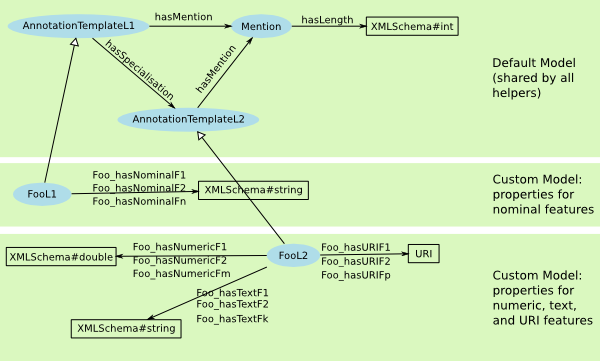
\includegraphics[scale=0.66]{img/dsah-model}
\caption{Default semantic annotation helper representation schema.}
\label{fig:dsah-model}
\end{center}
\end{figure}

The default generic SAH implementations try to minimise the amount of data stored in their underlying database or semantic repository
by creating representation templates that are shared
between all occurrences of annotations with the same values for the features.
There are two levels of templates, the first defined by the values of nominal
features, and the second that uses the values of all the other features. This
is intended to reflect the typical scenario where most annotations are defined
by a small set of nominal features, with a few of them having features with
arbitrary values. Most annotation types would then only make use of level-1
templates, with a few of them employing both level-1, and level-2 templates.

\begin{figure}[htb]
\begin{center}
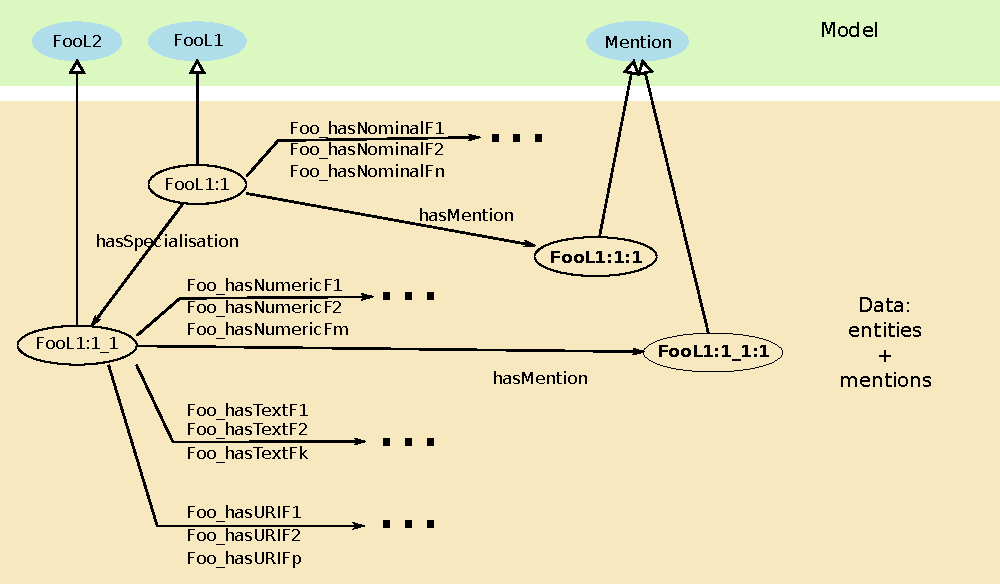
\includegraphics[scale=0.66]{img/dsah-data}
\caption{Default semantic annotation helper data example.}
\label{fig:dsah-data}
\end{center}
\end{figure}

The representation schema used by the Sesame helper is illustrated in
Figure~\ref{fig:dsah-model}.  Figure~\ref{fig:dsah-data} shows the data created
for an example annotation, with the two mention URIs displayed in bold. These
URIs will be stored in the mentions index.  The DB helper uses a similar
strategy, with separate level 1 (nominal) and level 2 (everything else)
database tables for each annotation type.  Annotation types that only have
nominal features need just a level 1 table.

The execution flow for each annotation includes the following main steps:
\bit
  \item Given the annotation's nominal features, find an appropriate level-1
  (L1) template. If none is found, create one.
  \item For the L1 template, find a mention of appropriate length (the number
  of tokens covered by the annotation). If none is found, create one. Add the
  mention URI to the mentions index.
  \item If the annotation has non-nominal features:
  \begin{itemize}
    \item Find an appropriate level-2 (L2) template, based on the feature
    values. If none is found, create one.
    \item For the L2 template, find (or create) a mention of appropriate length;
    add the mention URI to the index.
  \end{itemize}  
\eit

All annotations sharing the same feature values will share the same database
entries or knowledge base entities (the resources with URIs `\verb!FooL1:1!'
and `\verb!FooL1:1_1!'), and the same mention objects. This has the
advantage of reducing the size of the database, which allows more
documents to be indexed, and helps achieve better execution speeds during
search. The downside of this is that the indexing process is somewhat slowed
down, as pre-existing entities need to be retrieved at every step.
